\documentclass[10pt]{article}

\usepackage[utf8]{inputenc}
\usepackage{algorithmic}
\usepackage{algorithm}
\usepackage{pst-plot}
\usepackage{graphicx}
\usepackage{titlesec}
\titlespacing*{\section}
{0pt}{0ex plus 0ex minus 1ex}{0ex plus 0ex}
\titlespacing*{\subsection}
{0pt}{0ex plus 0ex minus 1ex}{0ex plus 0ex}
\usepackage{multicol}
\usepackage{endnotes}
\usepackage{graphics}
\usepackage{floatflt}
\usepackage{wrapfig}     
\usepackage{amsfonts}
\usepackage{amsmath}
\usepackage{verbatim}
\usepackage{hyperref}
\usepackage{multirow}
\usepackage{pdflscape}
\usepackage{color}
\usepackage[autostyle]{csquotes}
\usepackage{siunitx}
\usepackage{titling}
\usepackage{wrapfig}
\usepackage{geometry}
%%=========
\date{\vspace{-11.5ex}}
\author{\vspace{-10ex}}

\geometry{
    a4paper,
    total={170mm,257mm},
    left=0mm,
    right=0mm,
    top=0mm,
    bottom=0mm,
}

\usepackage{listings}
\usepackage{color}
 
\definecolor{codegreen}{rgb}{0,0.6,0}
\definecolor{codegray}{rgb}{0.5,0.5,0.5}
\definecolor{codepurple}{rgb}{0.58,0,0.82}
\definecolor{backcolour}{rgb}{0.95,0.95,0.92}
 
\lstdefinestyle{mystyle}{
    backgroundcolor=\color{backcolour},   
    commentstyle=\color{codegreen},
    keywordstyle=\color{blue},
    numberstyle=\tiny\color{codegray},
    stringstyle=\color{red},
    basicstyle=\footnotesize,
    breakatwhitespace=false,         
    breaklines=true,                 
    captionpos=b,                    
    keepspaces=true,                 
    numbers=left,                    
    numbersep=5pt,                  
    showspaces=false,                
    showstringspaces=false,
    showtabs=false,                  
    tabsize=2
}
 
\lstset{style=mystyle}
%%=========
\usepackage{footnote}
\makesavenoteenv{tabular}
\usepackage{gensymb}
\hypersetup{pdfborder={0 0 0 0}}

\pdfpagewidth 210mm
\pdfpageheight 297mm 
\setlength\topmargin{0mm}
\setlength\headheight{0mm}
\setlength\headsep{0mm}
\setlength\textheight{250mm}    
\setlength\textwidth{159.2mm}
\setlength\oddsidemargin{0mm}
\setlength\evensidemargin{0mm}
\setlength\parindent{7mm}
\setlength\parskip{0mm}


\author{Aqeel Labash}
\title{Bioinformatics}
\begin{document}
\maketitle
\section*{Task 1}
\subsection*{a) Merging to one dataset}
done that using this code (python): 
\begin{lstlisting}[language=python]
import pandas as pd
import matplotlib.pyplot as plt
import numpy as np
%matplotlib inline
dfa = pd.read_csv('pupila.csv',sep='\t')
dfc = pd.read_csv('pupilc.csv',sep='\t')
dfd = pd.read_csv('pupild.csv',sep='\t')
dfa['C'] = dfc['C']
dfa['D'] = dfd['D']
dfa.to_csv('ACD.csv',index=False)
\end{lstlisting}
\subsection*{b)Get Some heatmap}
\begin{lstlisting}[language=python]
ax = plt.subplot(1,1,1)
ax.pcolor(dfa[dfa.columns[[1,2,3]]].as_matrix())
ax.set_xticklabels(['','A','','C','','D',''])
plt.show()
\end{lstlisting}
\begin{figure}[H]
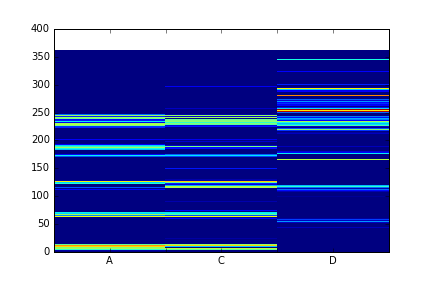
\includegraphics[scale=1]{heatmap.png}
\caption{Heat map of students}
\end{figure}
\subsection*{c)When Lessons Start}
For this actually I depended on the fact that usually during lessons people more focused on one thing so the activity of the student pupil should be much less.\\
So for the start,end times I would say : \\

\begin{tabular}{|c|c|c|}
\hline
\textbf{Class \#}&\textbf{School 1}&\textbf{School 2}\\
\hline
1 &8:15\(\rightarrow\)9:00&8:00\(\rightarrow\)8:45\\
\hline
2 &9:15\(\rightarrow\)10:00\footnote{Looks like there were some activity at the end of this class, activity started around 9:55 so I believe the class ended before the schedual}&9:00\(\rightarrow\)9:45\\
\hline
3 &10:15\(\rightarrow\)11:00\footnote{Seems starange time to start and end but make sense depending on the data. For accurate the class ended at 10:52}&10:00\(\rightarrow\)10:45\\
\hline
4 &11:10\(\rightarrow\)11:55\footnote{I selected this end depending on the class duration. but at the end of the class high activated does exist around 11:45}&11:00\(\rightarrow\)11:45 \footnote{This class contained some activity}\\
\hline
5&No movement on students \texttt{A,C}&12:00\(\rightarrow\)12:45\footnote{contained a lot of regular activate ( I think this one is the sport class}\\
\hline
6&No movement on students \texttt{A,C}&13:00\(\rightarrow\)13:45\\
\hline
\end{tabular}

\subsection*{1) Most active student}
\begin{lstlisting}[language=python]
dfa['A'].sum(),dfa['C'].sum(),dfa['D'].sum()
\end{lstlisting}
The previous code give :\texttt{A:5044, C:4663, D:4815)} we can notice that Student \texttt{A} was the most active student
\subsection*{2) Which two students from same school}
Students \texttt{A,C} were from the same class. Simply if we compare the active time we will find that students \texttt{A,C} values are highly correlated. 
\begin{lstlisting}[language=python]
dfa.corr()
\end{lstlisting}
\begin{table}[H]
\center
\begin{tabular}{|c|c|c|c|}
\hline
 &	A &	C 	&D \\
 	\hline
A &	1.000000 &	0.802555 	&0.052867\\
\hline
C 	&0.802555 	&1.000000 &	0.095510\\
\hline
D &	0.052867 &	0.095510 &	1.000000\\
\hline
\end{tabular}
\caption{Correlation between students pupils \label{table:1}}
\end{table}
From Table \ref{table:1} we can see how much students \texttt{A,C} are correlated.
\subsection*{3) Breakfast}
The breakfast for students \texttt{A,C} was from 8:05 \(\rightarrow\) 8:15 and for student \texttt{D} I think it's around 11:45 and 12:00 It might be a late breakfast but depending on what I noticed that breakfast is high pupile activity compared to other breaktime. Usually when we eat we use our eyes movement much more than using our nick so I guess that is the reason behind the high activity.
\subsection*{4) Which student has the physical class}
Student \texttt{D} has the physical class. This student has high pupil activity for long time.Fig. \ref{fig:2} show this activity in bottom left plot. Which make sense, since physical class student has to move his eye much more than traditional class.
\begin{lstlisting}[language=python]
plt.figure(figsize=(16,10))
ax = plt.subplot(2,2,1)
ax.set_title('Student A')
ax.set_xlabel('Minutes')
ax.set_ylabel('pupil activity')
ax.bar(dfa.index,dfa.A)
ax = plt.subplot(2,2,2)
ax.set_xlabel('Minutes')
ax.set_ylabel('pupil activity')
ax.bar(dfa.index,dfa.C)
ax.set_title('Student C')
ax = plt.subplot(2,2,3)
ax.set_xlabel('Minutes')
ax.set_ylabel('pupil activity')
ax.bar(dfa.index,dfa.D)
ax.set_title('Student D')
\end{lstlisting}

\begin{figure}[H]
\hspace{-70px}
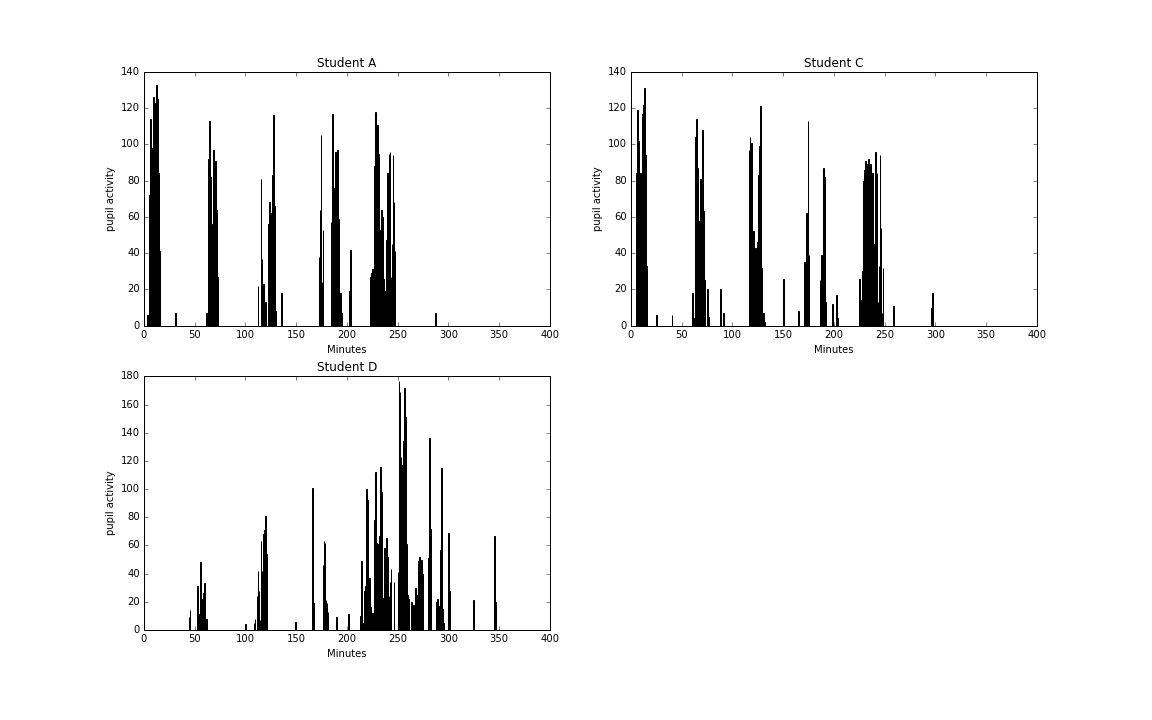
\includegraphics[scale=0.5]{bar.png}
\caption{bar plot for students activity \label{fig:2}}
\end{figure}
\subsection*{5) Difficulties with 100 students.}
Although we can see how things going with the current dataset, we don't know what actually happen. We might think that this less activity might be class but it might be just sleeping student :). On the large datasets we will have to deal with the noise of this kind all the way. The problem will be much harder with students from different classes and different schools (assuming untagged samples). I think one of the most problems will be detecting hardware deficit.
\section*{Task 2}
\subsection*{1)Most Expensive Bills}
\begin{lstlisting}[language=python]
df.sort(columns=['cost'],ascending=False).head()
\end{lstlisting}
Table \ref{table:3} show the most 3 expensive codes 
\begin{table}[H]
\center
\begin{tabular}{|c|c|}
\hline
\textbf{Code}&\textbf{Cost}\\
\hline
I22 &	11413.0\\
\hline
I21 &	6657.6\\
\hline
F20 &	4530.5\\
\hline
\end{tabular}
\caption{Most expensive codes \label{table:3}}
\begin{enumerate}
\item \textbf{I22 Subsequent myocardial infarction}
\begin{itemize}
\item I22.0 Subsequent myocardial infarction of anterior wall
\item I22.1 Subsequent myocardial infarction of inferior wall
\item I22.8 Subsequent myocardial infarction of other sites
\item I22.9 Subsequent myocardial infarction of unspecified site
\end{itemize}
\item \textbf{I21 Acute myocardial infarction}
\begin{itemize}
\item I21.0 Acute transmural myocardial infarction of anterior wall
\item I21.1 Acute transmural myocardial infarction of inferior wall
\item I21.2 Acute transmural myocardial infarction of other sites
\item I21.3 Acute transmural myocardial infarction of unspecified site
\item I21.4 Acute subendocardial myocardial infarction
\item I21.9 Acute myocardial infarction, unspecified 
\end{itemize}
\item \textbf{F20.0 Schizophrenia}
\begin{itemize}
\item F20.0 Paranoid schizophrenia
\item F20.1 Hebephrenic schizophrenia
\item F20.2 Catatonic schizophrenia
\item F20.3 Undifferentiated schizophrenia
\item F20.4 Post-schizophrenic depression
\item F20.5 Residual schizophrenia
\item F20.6 Simple schizophrenia
\item F20.8 Other schizophrenia  ( Cenesthopathic schizophrenia )
\item  F20.9 Schizophrenia, unspecified
\end{itemize}
\end{enumerate}
\end{table}

\subsection*{2) Max ICD10 by type}
\begin{lstlisting}[language=python]
sums = df.groupby(['icd10'])['cost'].sum()
sums.sort(inplace=True,ascending=False)
sums.head()
\end{lstlisting}
\begin{table}[H]
\center
\begin{tabular}{|c|c|}
\hline
\textbf{Code}&\textbf{Cost}\\
\hline
I22   & 17380.7\\
\hline
Z51   & 13958.6\\
\hline
F20   & 11575.7\\
\hline
\end{tabular}
\caption{Most expensive by Code sum\label{table:4}}
\end{table}
Table \ref{table:4} show the most expensive codes by total. Since we already saw \texttt{I22,F20} I'll just put deases names for \texttt{Z51}\\
\textbf{Z51 Other medical care}
\begin{itemize}
\item Z51.0 Radiotherapy session
\item Z51.1 Chemotherapy session for neoplasm
\item Z51.2 Other chemotherapy
\item Z51.3 Blood transfusion (without reported diagnosis)
\item Z51.4 Preparatory care for subsequent treatment, not elsewhere classified
\item Z51.5 Palliative care
\item Z51.6 Desensitization to allergens
\item Z51.8 Other specified medical care
\item Z51.9 Medical care, unspecified
\end{itemize}
\textbf{Note:} All code, .ipynb, .tex, .pdf etc... files could be found on \href{https://github.com/aqeel13932/BIO/tree/master/Pupils_HW}{github} specific files \href{https://github.com/aqeel13932/BIO/blob/master/Pupils_HW/Q1.ipynb}{Q1.ipynb} , \href{https://github.com/aqeel13932/BIO/blob/master/Pupils_HW/Q2.ipynb}{Q2.ipynb} \href{https://github.com/aqeel13932/BIO/blob/master/Pupils_HW/report.pdf}{PDF}
{\center \textbf{E.O.F\\ }}
\end{document}